% N2 view of a sequential aviation scenario, and of what MDO adds to it.
%
% Disciplines sit on the diagonal, in the order a sequential scenario runs them.
% A block's outputs leave along its row and enter the block they feed down its
% column, so everything above the diagonal flows forward and anything below it
% flows back. The reports' chain lives entirely above the diagonal; the
% cost-to-demand feedback is the one entry below it, and closing it is what an
% MDO solver does. Colours and blocks follow the AeroMAPS framework panel of the
% ATAG reproduction poster: teal for what the reports do, magenta for what they
% leave out, light blue for the blocks that carry the coupling.
%
% Build: pdflatex n2_sequential.tex  ->  n2_sequential.pdf
\documentclass[tikz,border=3pt]{standalone}
\usepackage[T1]{fontenc}
\usepackage[semibold]{sourceserifpro}
\usetikzlibrary{arrows.meta,calc}

\definecolor{panel}{HTML}{E9F8FF}
\definecolor{coupling}{HTML}{CBEEFF}
\definecolor{chainteal}{HTML}{0088B0}
\definecolor{soft}{HTML}{72B9D1}
\definecolor{navy}{HTML}{0A303E}
\definecolor{ink}{HTML}{201E1D}
\definecolor{added}{HTML}{D6006C}

\tikzset{
  disc/.style={draw=chainteal, line width=0.9pt, rounded corners=2pt, fill=white,
               minimum width=2.45cm, minimum height=1.08cm, align=center,
               inner sep=2pt, text=ink},
  carries/.style={disc, fill=coupling},
  background/.style={disc, draw=added, dashed, fill=panel},
  % Coupling variables: plain text on a translucent white patch, with no colour
  % of their own, so they read over the flows without being taken for one.
  cell/.style={draw=none, rounded corners=1.5pt, fill=white, fill opacity=0.95,
               text opacity=1, font=\scriptsize, align=center, inner sep=2.5pt,
               minimum height=0.55cm, text=ink},
  addcell/.style={cell},
  chain/.style={draw=chainteal, line width=1.1pt, -{Stealth[length=5pt,width=4pt]}},
  extra/.style={draw=added, line width=1.1pt, dash pattern=on 4pt off 2.5pt,
                -{Stealth[length=5pt,width=4pt]}},
}

% title and subtitle of a diagonal block
\newcommand{\block}[2]{{\small\bfseries\color{navy}#1}\\[-1pt]{\scriptsize #2}}

\begin{document}
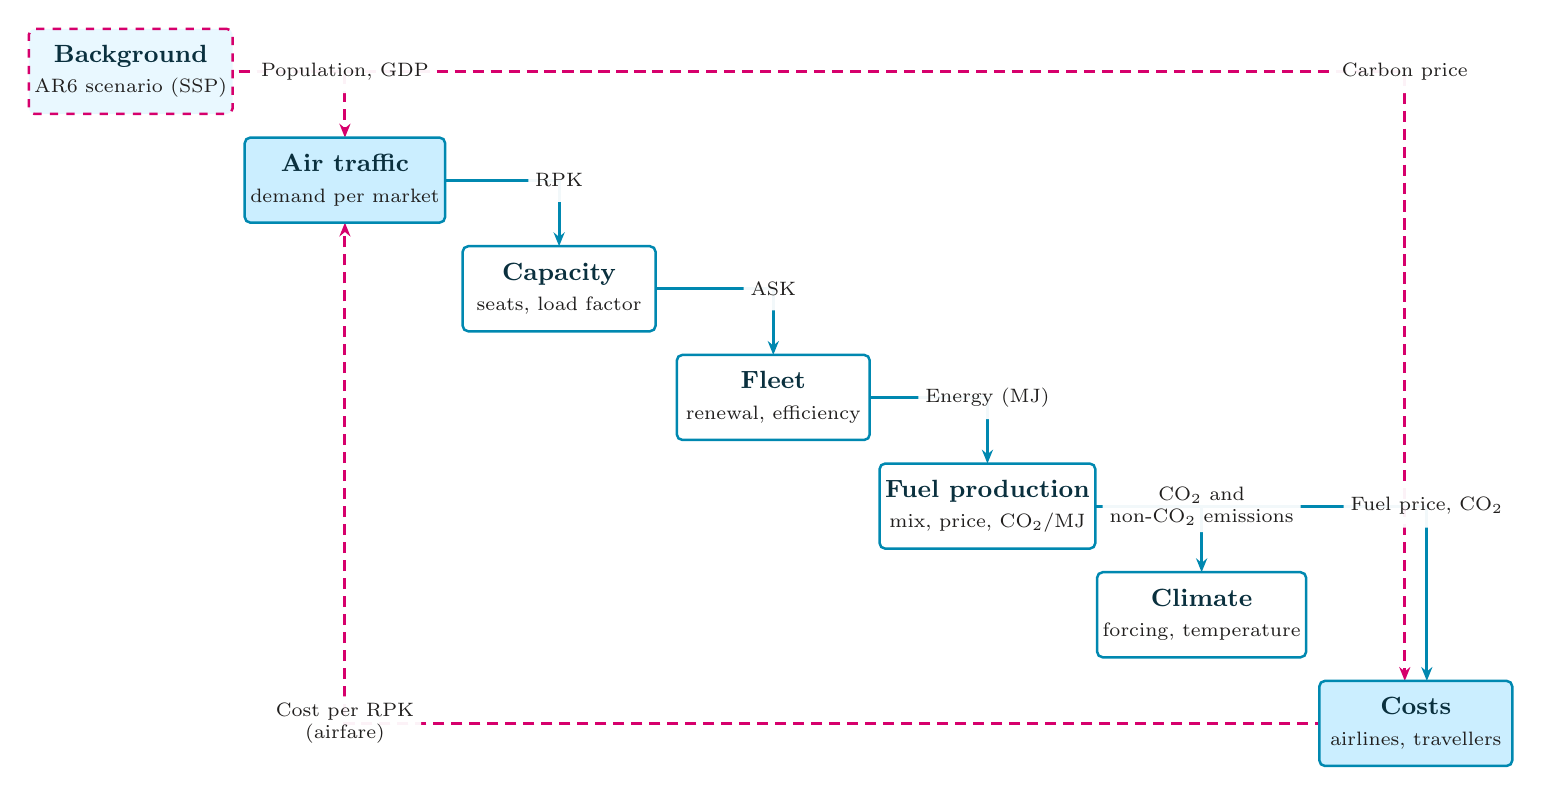
\begin{tikzpicture}
  \def\dx{2.72}
  \def\dy{1.38}
  \def\half{0.54}   % half the block height: where a flow meets a block
  \def\lane{0.14}   % offset of the two flows sharing column 6

  % p<k> is the diagonal position of discipline k; the coupling cell in row r
  % and column c is then (p<c> |- p<r>).
  \foreach \k in {0,...,6} {\coordinate (p\k) at (\k*\dx, -\k*\dy);}

  % --- data flows, drawn first so the blocks sit on top ---------------------
  % sequential chain, above the diagonal
  \draw[chain] (p1) -| ($(p2)+(0,\half)$);
  \draw[chain] (p2) -| ($(p3)+(0,\half)$);
  \draw[chain] (p3) -| ($(p4)+(0,\half)$);
  \draw[chain] (p4) -| ($(p5)+(0,\half)$);
  % Column 6 carries two inputs, the fuel price from row 4 and the carbon price
  % from row 0; they run a hair apart so the dashed one stays readable.
  \draw[chain] (p4) -| ($(p6)+(\lane,\half)$);
  % background scenario, added here
  \draw[extra] (p0) -| ($(p1)+(0,\half)$);
  \draw[extra] (p0) -| ($(p6)+(-\lane,\half)$);
  % cost-to-demand feedback, below the diagonal: closed by MDO
  \draw[extra] (p6) -| ($(p1)+(0,-\half)$);

  % --- coupling variables, one cell per link -------------------------------
  \node[addcell] at (p1 |- p0) {Population, GDP};
  \node[addcell] at ($(p6 |- p0)+(-\lane,0)$) {Carbon price};
  \node[cell] at (p2 |- p1) {RPK};
  \node[cell] at (p3 |- p2) {ASK};
  \node[cell] at (p4 |- p3) {Energy (MJ)};
  \node[cell] at (p5 |- p4) {CO$_2$ and\\non-CO$_2$ emissions};
  \node[cell] at ($(p6 |- p4)+(\lane,0)$) {Fuel price, CO$_2$};
  \node[addcell] at (p1 |- p6) {Cost per RPK\\(airfare)};

  % --- disciplines on the diagonal -----------------------------------------
  \node[background] at (p0) {\block{Background}{AR6 scenario (SSP)}};
  \node[carries]    at (p1) {\block{Air traffic}{demand per market}};
  \node[disc]       at (p2) {\block{Capacity}{seats, load factor}};
  \node[disc]       at (p3) {\block{Fleet}{renewal, efficiency}};
  \node[disc]       at (p4) {\block{Fuel production}{mix, price, CO$_2$/MJ}};
  \node[disc]       at (p5) {\block{Climate}{forcing, temperature}};
  \node[carries]    at (p6) {\block{Costs}{airlines, travellers}};

\end{tikzpicture}
\end{document}
